\hypertarget{group__ligands__up}{}\section{Ligands binding to unstructured domains}
\label{group__ligands__up}\index{Ligands binding to unstructured domains@{Ligands binding to unstructured domains}}


Add ligand binding to loop regions using the \hyperlink{group__domains__up}{Unstructured domains} feature.  


Add ligand binding to loop regions using the \hyperlink{group__domains__up}{Unstructured domains} feature. 

Sometime, certain ligands, like single strand binding (S\+SB) proteins, compete with intramolecular base pairing of the R\+NA. In situations, where the dissociation constant of the ligand is known and the ligand binds to a consecutive stretch of single-\/stranded nucleotides we can use the \hyperlink{group__domains__up}{Unstructured domains} functionality to extend the R\+NA folding grammar. This module provides a convenience default implementation that covers most of the application scenarios.

The function \hyperlink{group__domains__up_gaec0c3313fb2951946614f920d289829a}{vrna\+\_\+ud\+\_\+add\+\_\+motif()} attaches a ligands sequence motif and corresponding binding free energy to the list of known ligand motifs within a \hyperlink{group__fold__compound_a4f70b6d32681fc8ca061236f21819ae7}{vrna\+\_\+fold\+\_\+compound\+\_\+t.\+domains\+\_\+up} attribute. The first call to this function initializes the \hyperlink{group__domains__up}{Unstructured domains} feature with our default implementation. Subsequent calls of secondary structure predciction algorithms with the modified \hyperlink{group__fold__compound_ga1b0cef17fd40466cef5968eaeeff6166}{vrna\+\_\+fold\+\_\+compound\+\_\+t} then directly include the competition of the ligand with regules base pairing. Since we utilize the unstructured domain extension, The ligand binding model can be removed again using the \hyperlink{group__domains__up_gada59cb0c498b812eadd010811af3f2d4}{vrna\+\_\+ud\+\_\+remove()} function. Collaboration diagram for Ligands binding to unstructured domains\+:
\nopagebreak
\begin{figure}[H]
\begin{center}
\leavevmode
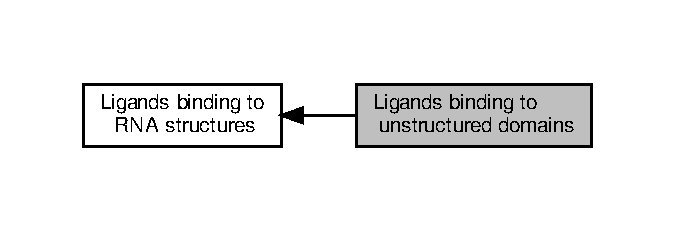
\includegraphics[width=324pt]{group__ligands__up}
\end{center}
\end{figure}
